\documentclass{beamer}
\mode<presentation>
{
  \usetheme{Madrid}      % or try Darmstadt, Madrid, Warsaw, ...
  \usecolortheme{dolphin} % or try albatross, beaver, crane, ...
  \usefonttheme{default}  % or try serif, structurebold, ...
  \setbeamertemplate{navigation symbols}{}
  \setbeamertemplate{caption}[numbered]
} 

\usepackage[english]{babel}
\usepackage[utf8]{inputenc}
\usepackage[T1]{fontenc}

\title[Wikidata WikiProject COVID-19]{Wikidata WikiProject COVID-19}
\author[User:TiagoLubiana]{Tiago Lubiana - University of São Paulo}
\date[25/06/2020]{June 25th, 2020}


\begin{document}

\begin{frame}
  \titlepage
\end{frame}

% Uncomment these lines for an automatically generated outline.
%\begin{frame}{Outline}
%  \tableofcontents
%\end{frame}


\section{Intro}

\begin{frame}{Quick intro to Wikidata}

\begin{itemize}
    \item Wikidata is a Wikimedia project that wants to \textit{structure} infos on Wikipedia
\end{itemize}

\begin{figure}
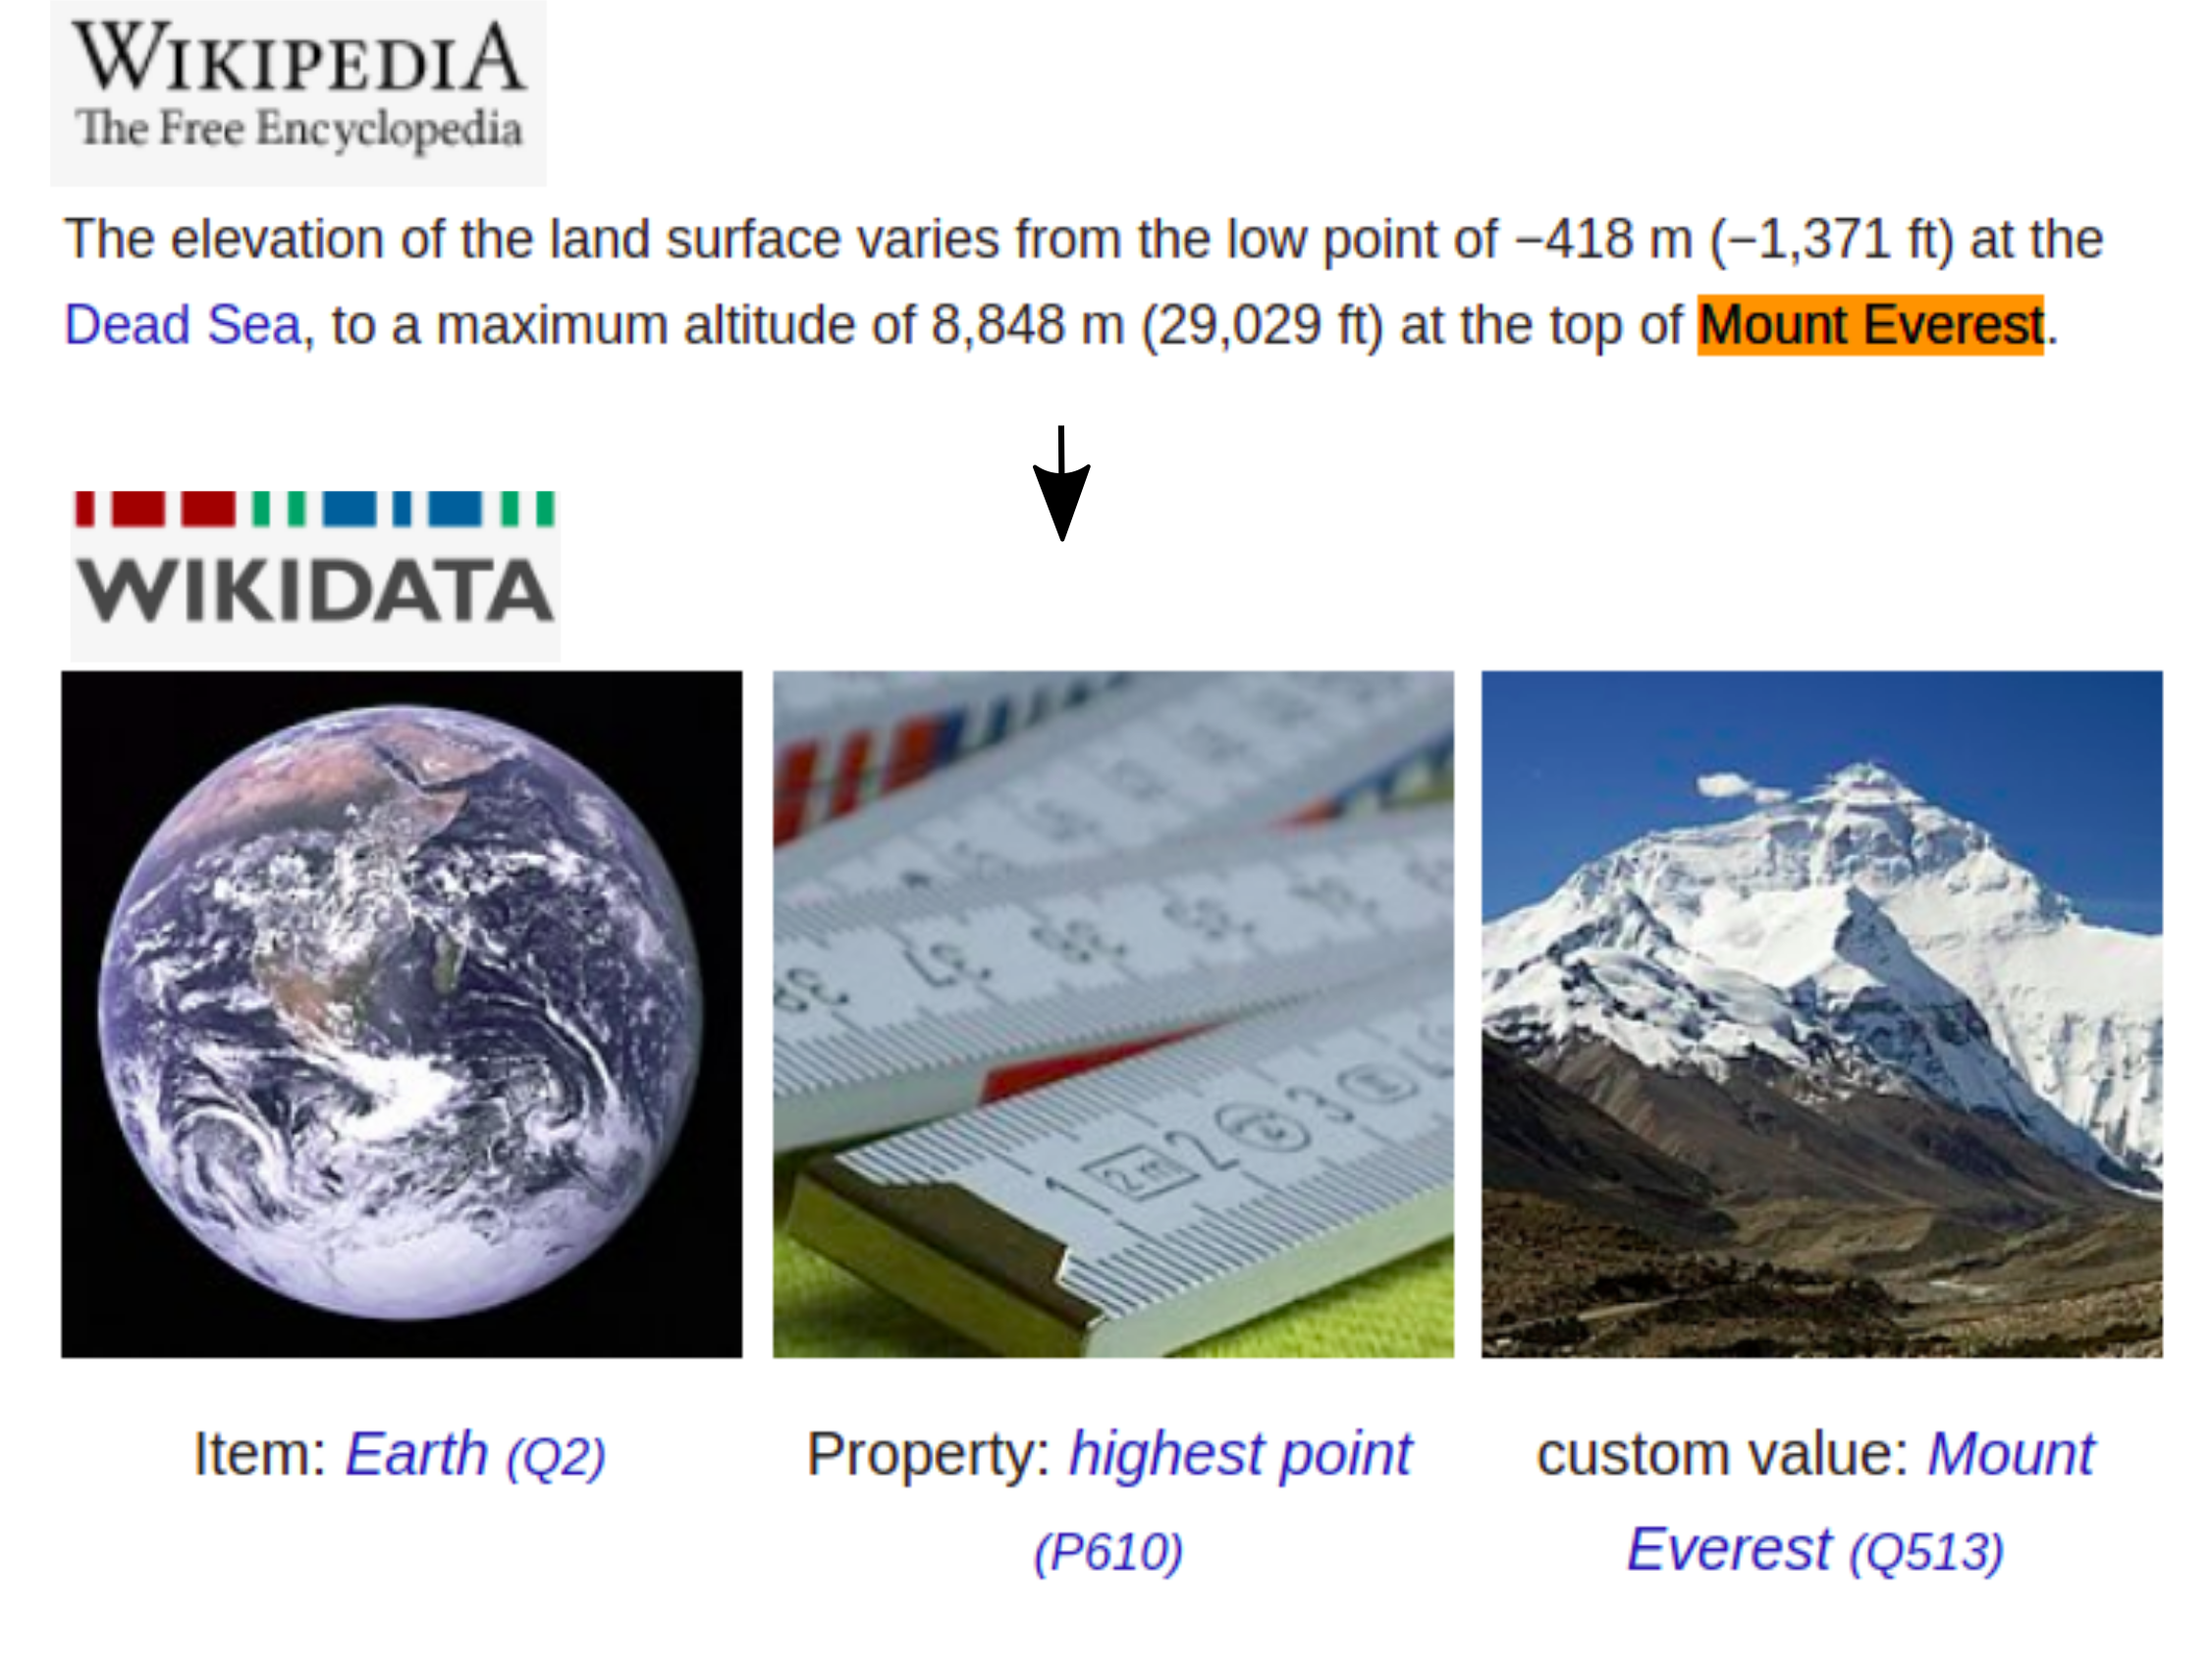
\includegraphics[scale=0.45]{fig/intro wikidata.png}
\end{figure}

\end{frame}


\begin{frame}{Quick intro to Wikidata}

\begin{itemize}
    \item Wikidata's structure is similar to a RDF triplestore
\end{itemize}
\begin{figure}

\includegraphics[scale=0.45]{fig/item_property_value.png}
\end{figure}

\end{frame}


\begin{frame}{Quick intro to Wikidata}

\begin{itemize}
    \item Relationship to Wikipedia
    
    \begin{itemize}
        \item Wikipedia already has structured data, but in suboptimal format
    \end{itemize}
    
\end{itemize}

\begin{figure}
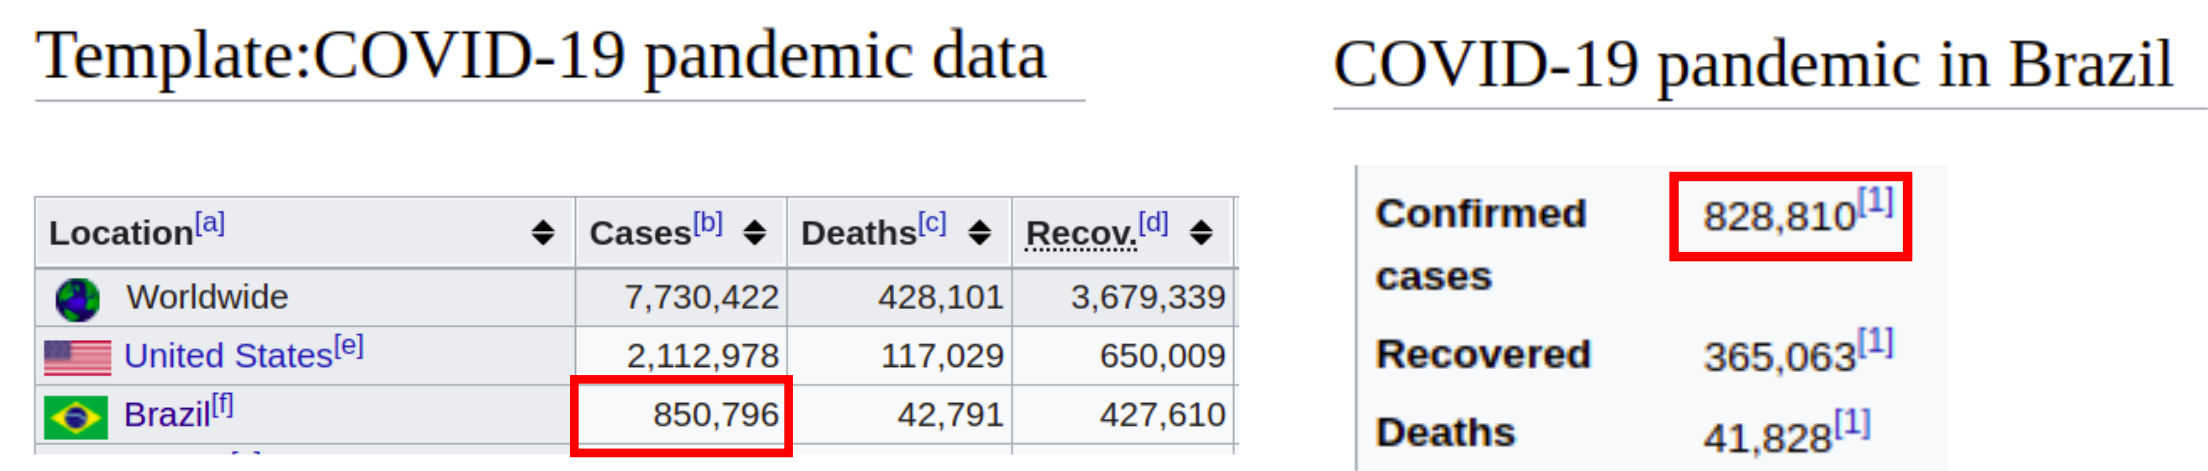
\includegraphics[scale=0.45]{fig/template_covid_19_brasil.png}
\end{figure}
and this is only one out of 309 different languages!
\end{frame}


\begin{frame}{Quick intro to Wikidata}

\begin{itemize}
    \item Relationship to Wikipedia
    
    \begin{itemize}
        \item Moving structured data to Wikidata enables wide and reliable reuse
    \end{itemize}
    
\end{itemize}

\begin{figure}
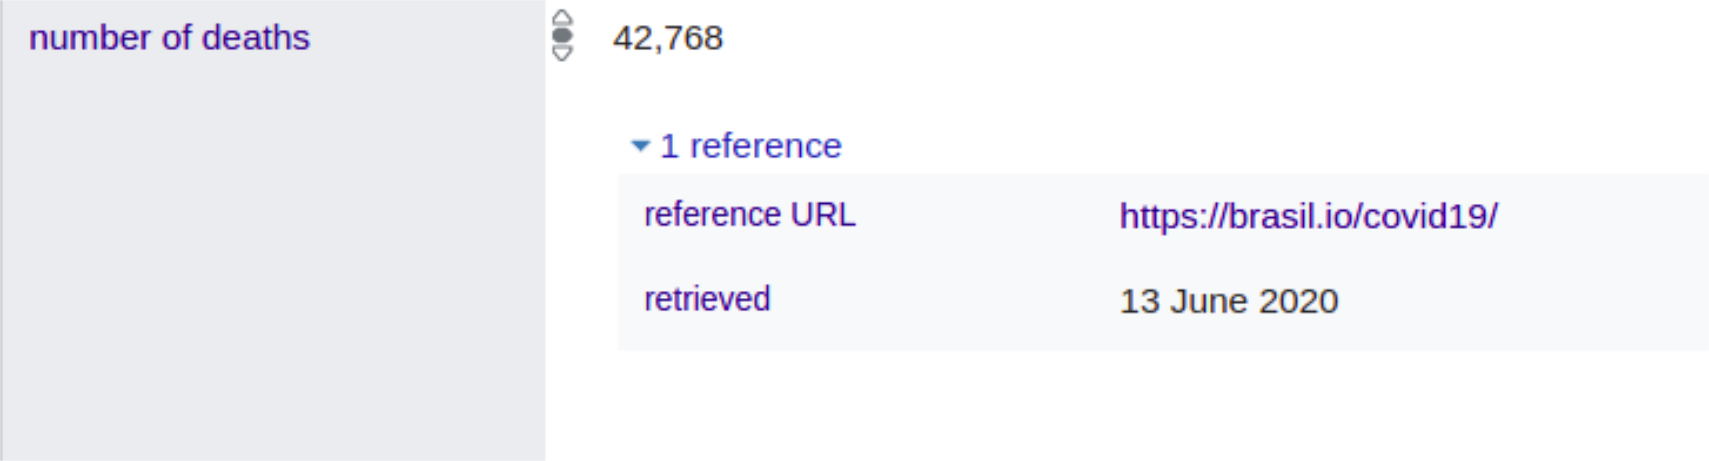
\includegraphics[scale=0.45]{fig/covid_19_brasil_on_wikidata.png}
\end{figure}
\end{frame}



\begin{frame}{Wikiprojects}

\begin{itemize}
    \item WikiProjects are groups of contributors who want to work together as a team to improve Wikidata.
    \item Focus on specific tasks or areas
    \item Know more about projects and quality metrics, check Wikidata Lab XVI 
    
\end{itemize}
\vskip 3cm
\url{https://pt.wikipedia.org/wiki/Wikip\%C3\%A9dia:Edit-a-thon/Atividades_em_portugu\%C3\%AAs/Wikidata_Lab_XVI}

\end{frame}


\begin{frame}{Wikiprojects}

\begin{itemize}
    \item There are Wikiprojects about a great variety of topics:
    \begin{itemize}
        \item Wikidata:WikiProject\_Books
        \item Wikidata:WikiProject\_Ancient\_Rome
        \item Wikidata:WikiProject\_Biology
        \item Wikidata:WikiProject\_Schemas
    \end{itemize}
\vskip 1cm
\end{itemize}
And anyone can get envolved!

\end{frame}

\begin{frame}{Wikiproject COVID-19 - Overview}

\begin{itemize}
    \item A group of users working to structure information about the COVID-19 pandemic at Wikidata.
    \item Project was created on 16 of March.
    \item +50 participants from all over the world.
\end{itemize}

\begin{figure}
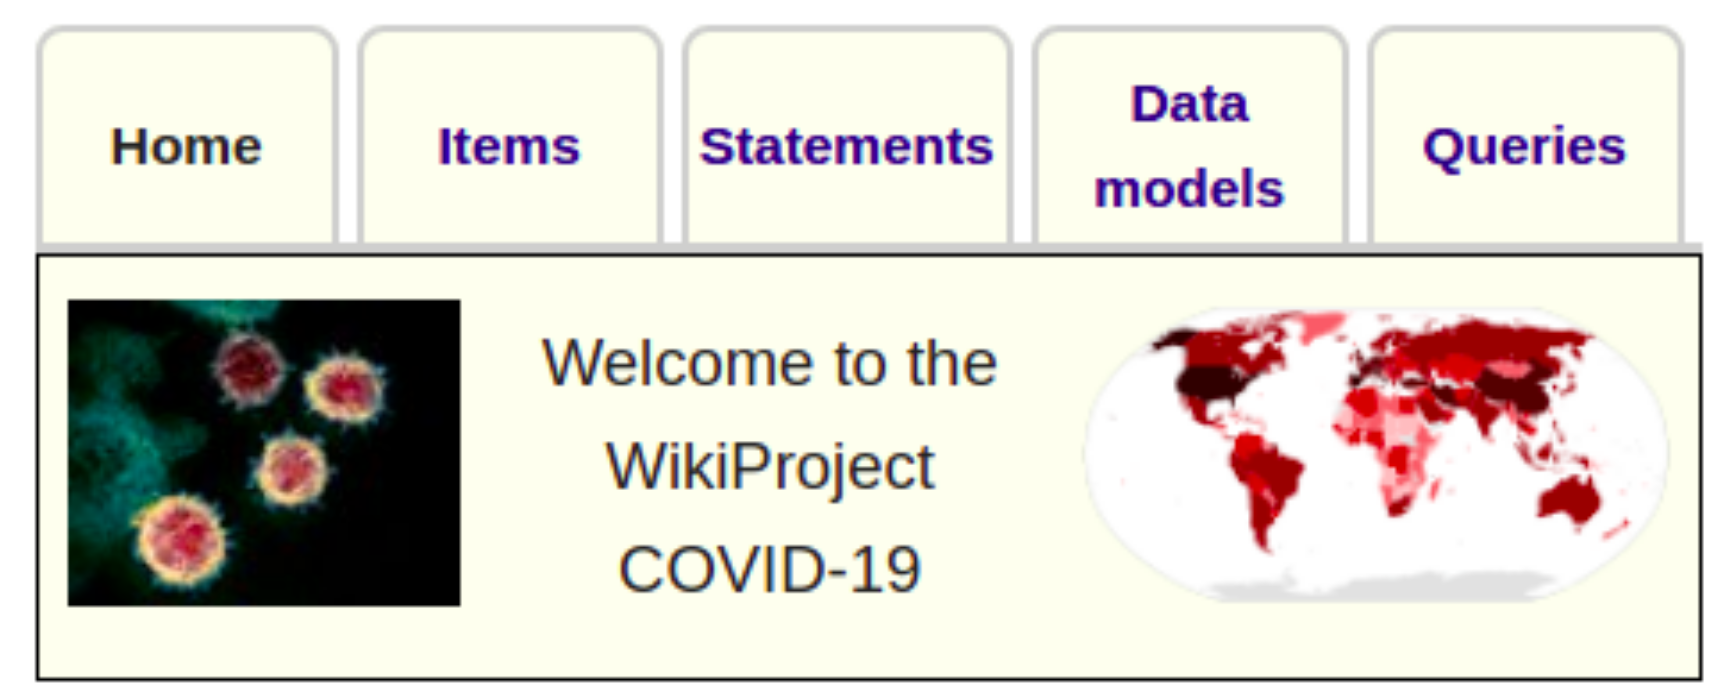
\includegraphics[scale=0.65]{fig/covid_banner.png}
\end{figure}
\vskip 2cm

\url{wikidata.org/wiki/Wikidata:WikiProject_COVID-19}

\end{frame}

\begin{frame}{Wikiproject COVID-19 - Overview}

\begin{itemize}
    \item Motivations behind the WikiProject:
    \begin{itemize}
        \item Data quality monitoring and data modeling for a quickly evolving situation
        \item "Oiling the machine" for future crises
        \item Standardization of data accross Wikipedias. 
        \item Providing structured data for secondary visualizations
    \end{itemize}
\end{itemize}

\url{wikidata.org/wiki/Wikidata:WikiProject_COVID-19}

\end{frame}


\begin{frame}{Wikiproject COVID-19 - Quality monitoring and modelling}
\begin{itemize}
    \item Collaborative approach
    \item Bottom-up, iterative process
\end{itemize}
\end{frame}


\begin{frame}{Wikiproject COVID-19 - "Oiling the machine"}
\begin{itemize}
    \item Create new data models 
    \item Improve the process itself of creating the model
    \item Finding consensus
    \item Expressing constraints
    \item Monitoring item quality
\end{itemize}
\end{frame}

\begin{frame}{Wikiproject COVID-19 - Standardization of Wikipedias}

\begin{itemize}
    \item Open problem: standardization. 
    \item Examples of different approaches for number of cases :
    \begin{itemize}
        \item Q83873593 (France) 
        \item Q84081576 (Sweden)
    \end{itemize}
\end{itemize}
\end{frame}

\begin{frame}{Wikiproject COVID-19 - Providing structured data for secondary visualizations}
\begin{itemize}
    \item Wikidata Queries using the SPARQL system 
    \item External databases that use Wikidata COVID-19 data.
\end{itemize}
\end{frame}



\begin{frame}{Wikiproject COVID-19 - Data Models (schemas) }
\begin{itemize}
    \item Example:https://www.wikidata.org/wiki/Wikidata:WikiProject\_COVID-19/Data\_models/Outbreaks
    \item Properties and human-readable models
    \item ShEx and computer readable models
\end{itemize}
\end{frame}

\begin{frame}{Wikiproject COVID-19 - Data Models (sources)}
\begin{itemize}
    \item Reuse of Wikidata properties
    \item Inspirations in external modelling approaches
\end{itemize}
\end{frame}

\begin{frame}{Wikiproject COVID-19 - Data Models (community)}
\begin{itemize}
    \item Who creates a data model?
    \item Where the discussions happen?
    \item How is consensus reached?
    \begin{itemize}
        \item Data models are innocent until proven otherwise.
    \end{itemize}
    \item How are these models enforced?
\end{itemize}
\end{frame}

\begin{frame}{Wikiproject COVID-19 - Data Models (community)}
\begin{itemize}
    \item If something is not modelled for other use cases, how to insert this on Wikidata?
    \item Property Proposals and Wikidata Property Admins.
\end{itemize}
\end{frame}

\begin{frame}{Diving into ShEx)}
\begin{itemize}
    \item Language for data structures
    \item ShEx core, optional properties and so on
    \item Tools to generate ShEx and validate Wikidata items
\end{itemize}
\end{frame}


\begin{frame}
  \titlepage
\end{frame}

\end{document}